%%%%%%%%%%%%%%%%%%%%%%
\begin{frame}{System description}

  \begin{columns}
   \begin{column}{.50\textwidth}
  	\begin{center}
      The system we are going to analyze is a simplified example of a
      {\textcolor{green!40!black}{\fontsize{13}{15}\textbf{surveillance system}}}
      for a restaurant.

      \vskip 0.5cm

      The system must notify to the owner and to the people nearby when someone
      tries to break in and enter in the restaurant in order to steal goods or
      damage the equipment.
  	\end{center}
   \end{column}

   \begin{column}{.50\textwidth}
  	\begin{center}
      \begin{figure}[ht!]
        \centering
        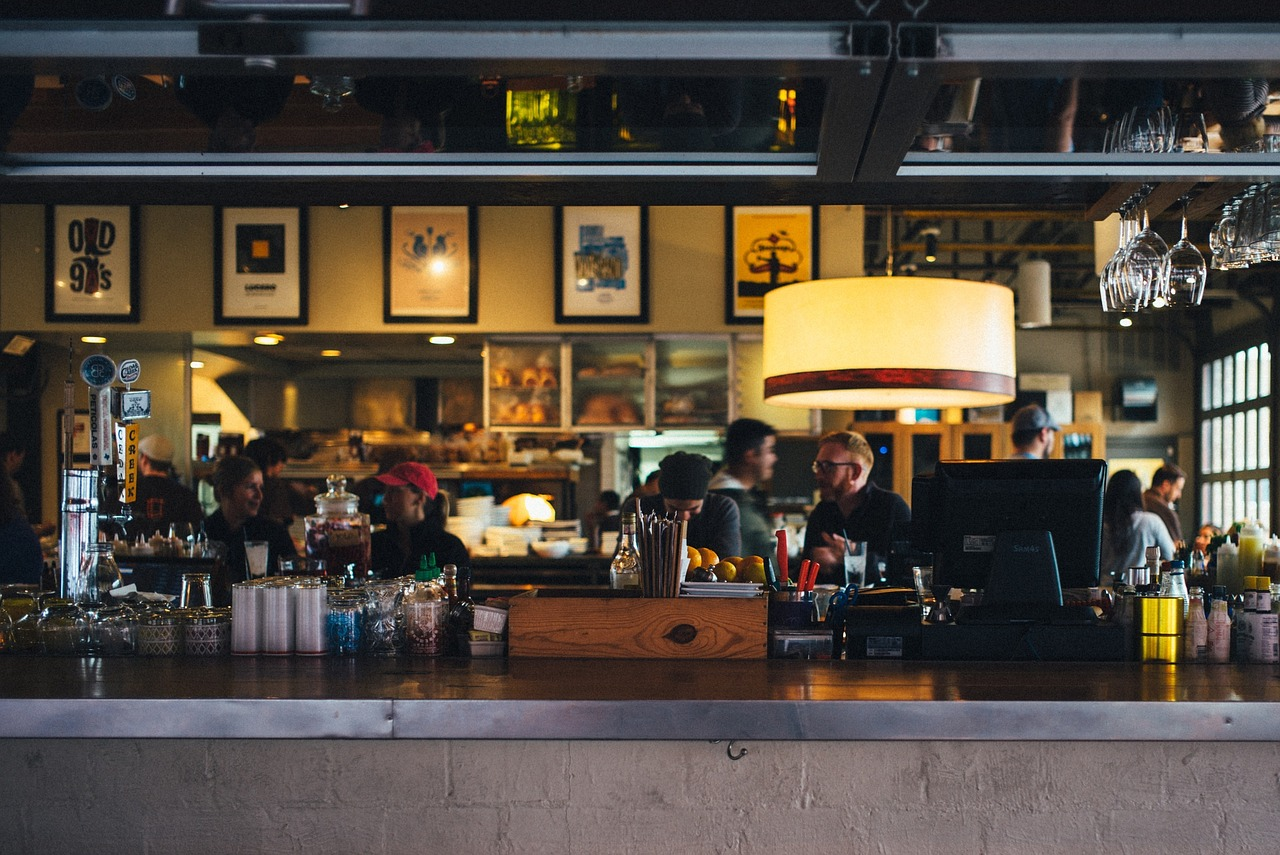
\includegraphics[width=50mm]{images/Alarm.jpg}
        \caption{Source: Alarm.org}
      \end{figure}
  	\end{center}
  	\vskip 0.3cm
   \end{column}
 \end{columns}

\end{frame}

%%%%%%%%%%%%%%%%%%%%%%
\begin{frame}{Main functions}

  \begin{columns}
   \begin{column}{.50\textwidth}
      1) The main function of the system, when active, is to signal eventual
      intruders with phone calls and acoustic signals from the sirens.

      \begin{figure}[ht!]
        \centering
        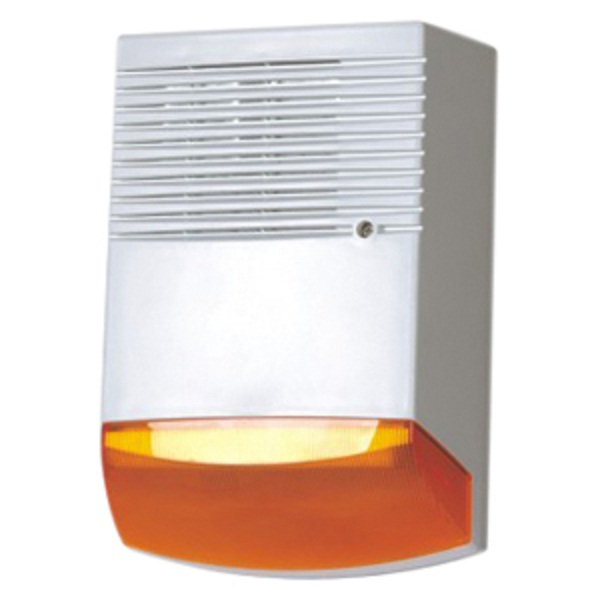
\includegraphics[width=30mm]{images/siren.jpg}
        \caption{Source: bizspia.org}
      \end{figure}

   \end{column}

   \begin{column}{.50\textwidth}
   \vskip 0.1cm

   \begin{figure}[ht!]
     \centering
     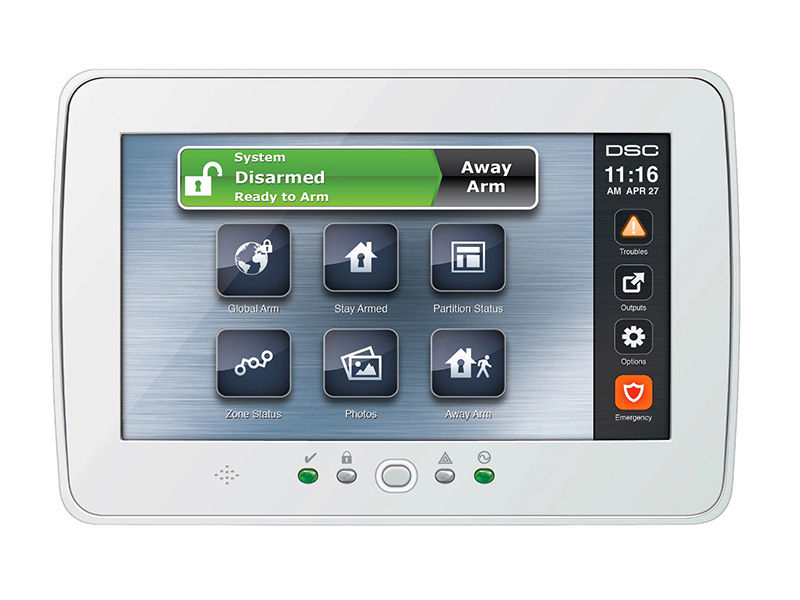
\includegraphics[width=30mm]{images/dsc.jpg}
     \caption{Source: dsc.com}
   \end{figure}

   \vskip 0.1cm
   2) It must be possible for authorized people to disable the system,
   either locally or using a remote procedure.
   \end{column}
 \end{columns}

\end{frame}

%%%%%%%%%%%%%%%%%%%%%%
\begin{frame}{Focus of the analysis}

  \begin{columns}
   \begin{column}{.50\textwidth}
      The objective of the analysis is to provide a description
      of the system hazards from an
      {\textcolor{green!40!black}{\fontsize{13}{15}\textbf{high level point of view}}},
      considering the main components as atomic.

      \vskip 0.8cm

      In this way we avoid the complexity of the analysis of the subcomponents,
      but we can focus only on the functionalities offered to the users.

   \end{column}

   \begin{column}{.50\textwidth}
   \vskip 0.3cm

   \begin{figure}[ht!]
     \centering
     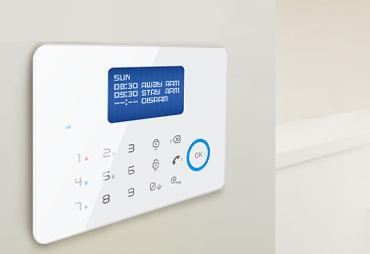
\includegraphics[width=50mm]{images/keypad.jpg}
     \caption{Source: DHgate.com}
   \end{figure}

   \end{column}
 \end{columns}

\end{frame}

%%%%%%%%%%%%%%%%%%%%%%
\begin{frame}{General system overview}

  \begin{columns}
   \begin{column}{.50\textwidth}
      The {\textcolor{green!40!black}{\fontsize{13}{15}\textbf{main}}}
       hardware and software
       {\textcolor{green!40!black}{\fontsize{13}{15}\textbf{components}}}
        of the system are presented
      in the following list:
      \begin{itemize}
        \item Central unit
        \item Infrared sensors
        \item Magnetic contacts
        \item Internal and external sirens
        \item Telephone module
        \item Alarm module
        \item Output modules
        \item User access points
      \end{itemize}
   \end{column}

   \begin{column}{.50\textwidth}
   \vskip 0.3cm
   \begin{center}
      \begin{figure}[ht!]
        \centering
        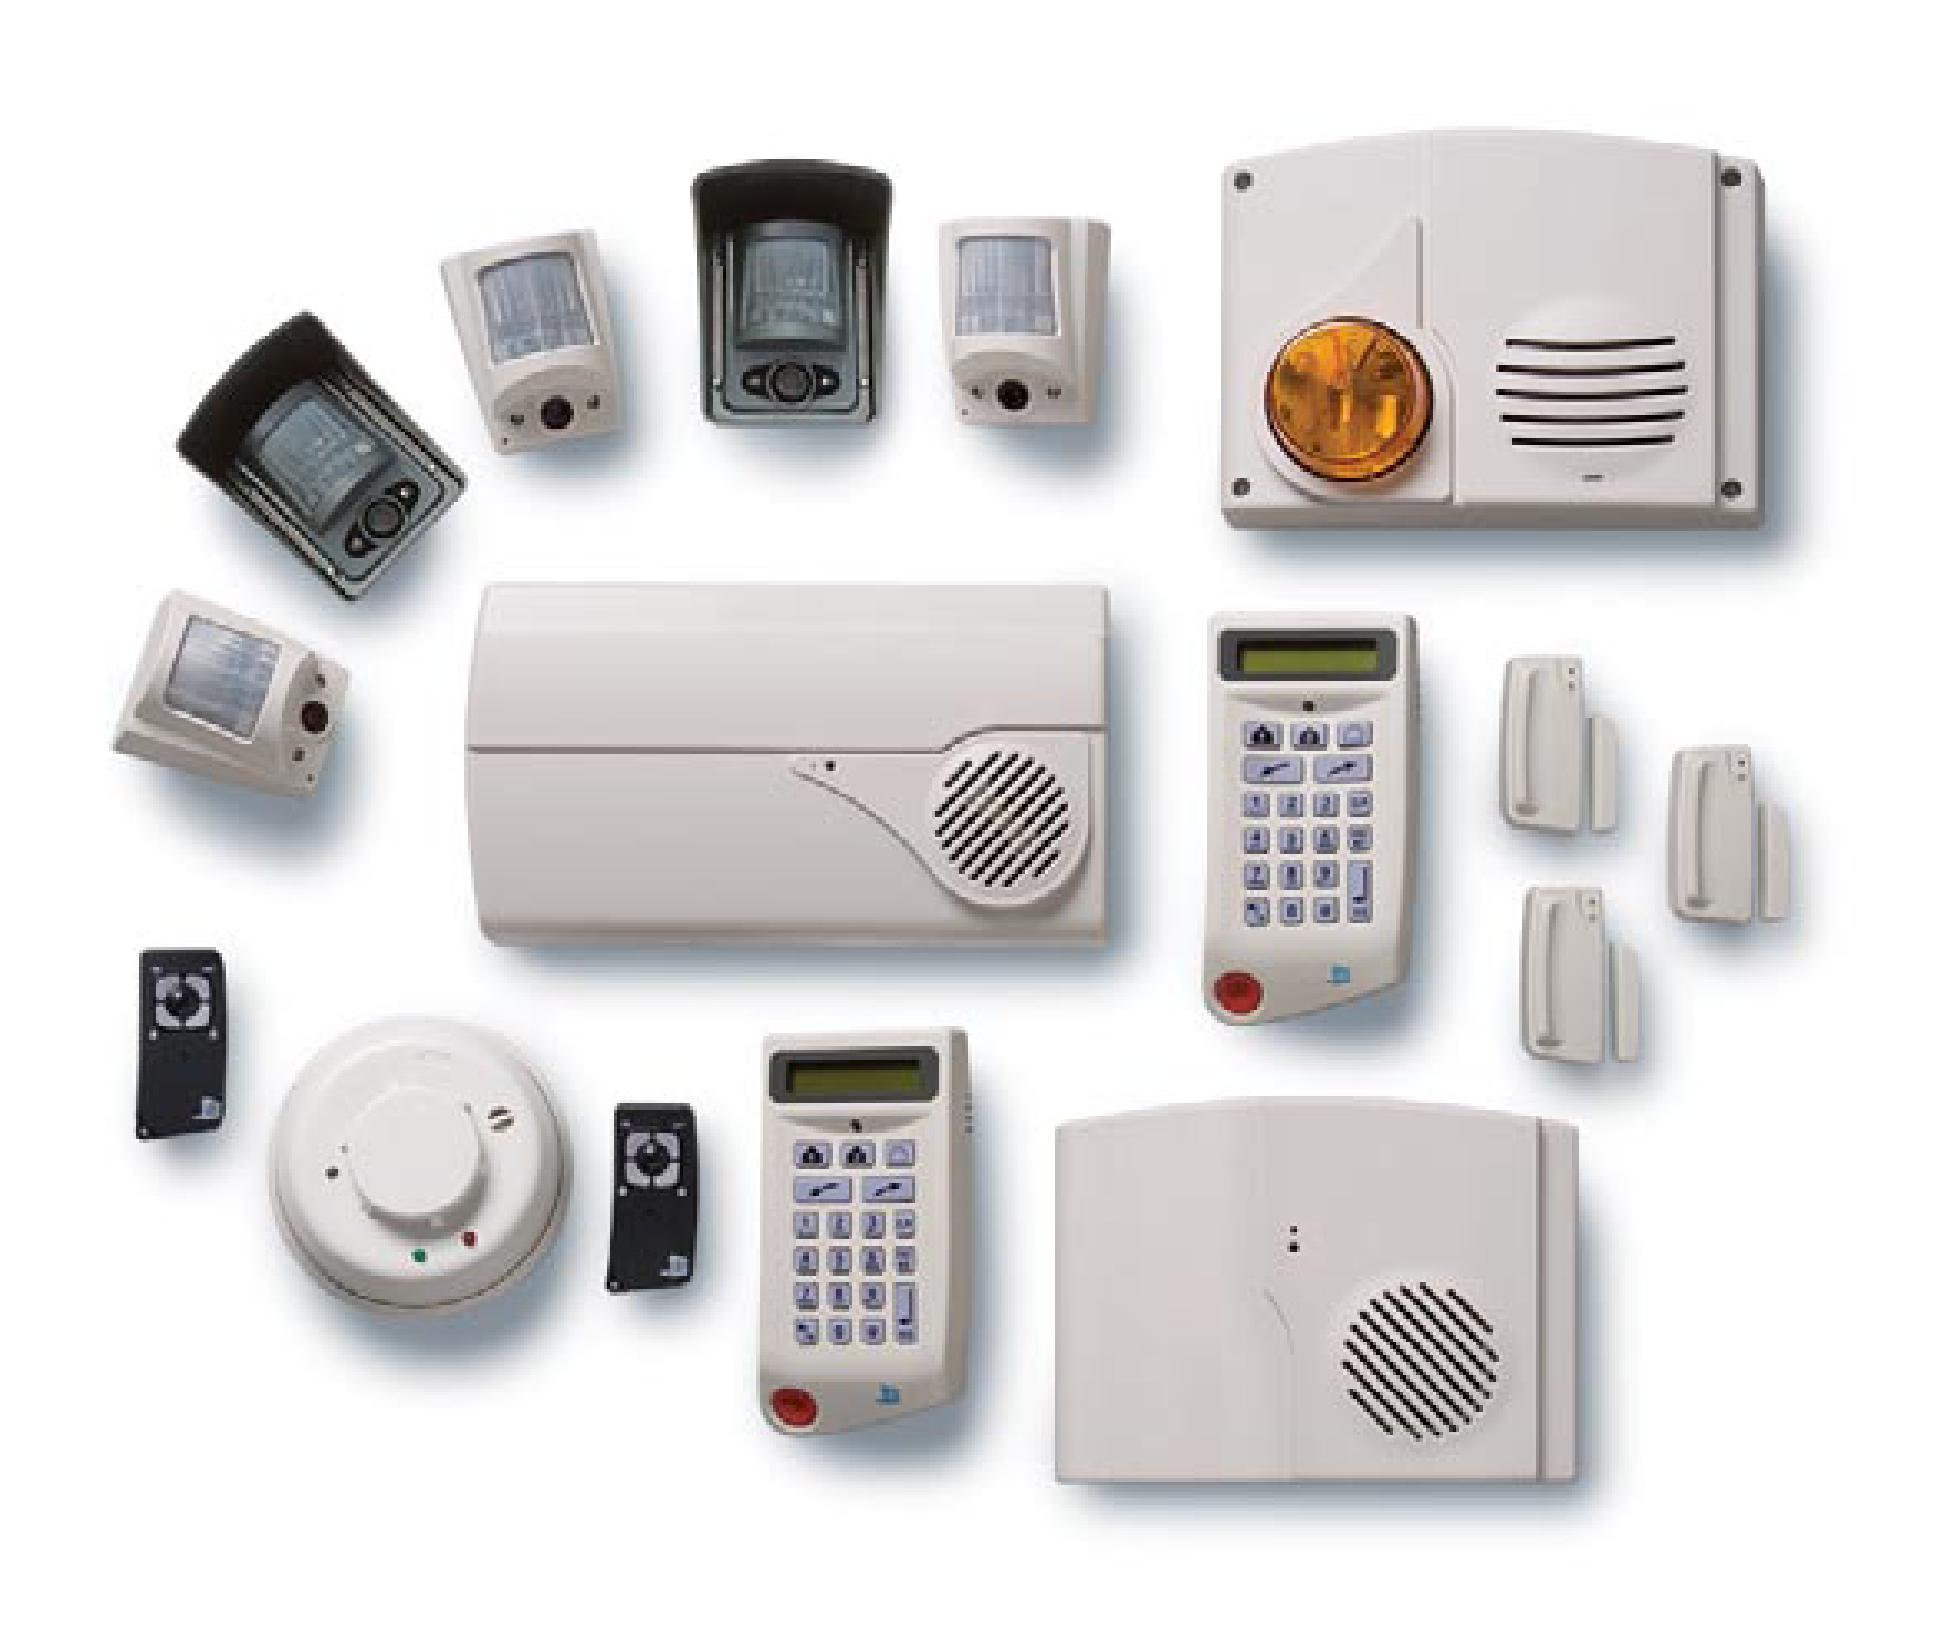
\includegraphics[width=60mm]{images/alarm_systems.jpg}
        \caption{Source: coreportal.org}
      \end{figure}
   \end{center}
   \end{column}
 \end{columns}

\end{frame}

%%%%%%%%%%%%%%%%%%%%%%
\begin{frame}{Components}

  \begin{columns}
   \begin{column}{.50\textwidth}
    The {\textcolor{green!40!black}{\fontsize{13}{15}\textbf{Central unit}}}
    controls all the system and offers the power supply to all the components.
      \vskip 0.3cm

    The {\textcolor{green!40!black}{\fontsize{13}{15}\textbf{infrared sensors
    and the magnetic contacts}}}
    protect the openings and the rooms of the building.
      \vskip 0.3cm

    The {\textcolor{green!40!black}{\fontsize{13}{15}\textbf{two sirens}}},
    one internal and one external, signal a perceived intrusion through
    acoustic advices.

      \vskip 0.3cm

    The {\textcolor{green!40!black}{\fontsize{13}{15}\textbf{telephone module}}}
    is in charge to make phone calls whenever an alarm is detected.

   \end{column}

   \begin{column}{.50\textwidth}
    The {\textcolor{green!40!black}{\fontsize{13}{15}\textbf{alarm module}}}
    receives the perceptions of the sensors and decides whether there is
    an intrusion or not. It also communicates with the sirens and
    the telephone module.

     \vskip 0.3cm

    The {\textcolor{green!40!black}{\fontsize{13}{15}\textbf{output module}}}
    informs the user about the state of the system, using leds.

     \vskip 0.3cm

    The {\textcolor{green!40!black}{\fontsize{13}{15}\textbf{user access points}}}
    allow the user to login and change the state of the system.
   \end{column}
 \end{columns}

\end{frame}
